\documentclass[11pt]{article}

\usepackage[utf8]{inputenc}
\usepackage{tabularx}
\usepackage{hyperref}
\usepackage{array}  
\usepackage{graphicx}
\usepackage{geometry}
\usepackage{fancyhdr}
\usepackage{tikz}
\usepackage{anyfontsize}
\usepackage[table,xcdraw]{xcolor}
\usepackage{tabularx, etoolbox}
\usepackage{eso-pic} 
\usepackage{float}

\newcommand\version{0.4.1} %aggiunta versione come variabile

\graphicspath{{images/}}
%\graphicspath{{../images/}}

%cambio misure della pagina
\geometry{a4paper,left=20mm,right=20mm,top=20mm}
%ebdfc7
\definecolor{colorePie}{HTML}{ebdfc7}


\pagestyle{fancy}
\fancyhf{}
\renewcommand{\headrulewidth}{0.4pt}
\lhead{
    \parbox[c]{1cm}{\includegraphics[width=1.1cm]{Sevenbitslogo.png}}
}
\rhead{\textcolor[HTML]{9e978a}{ Piano di Progetto v\version}
}
\setlength{\headheight}{25pt}
\cfoot{\thepage}


\renewcommand*\contentsname{Indice}
\renewcommand{\listfigurename}{Elenco delle figure}

\begin{document}

% Pagina del titolo
\begin{titlepage}
    \setcounter{page}{0}
    \centering
    % Inserisci il logo del gruppo (modifica il percorso dell'immagine)
    \includegraphics[width=7.2cm]{Sevenbitslogo.png} \\[2cm] 
    
    % Titolo
     {\fontsize{40}{40}\bfseries Piano di Progetto}\selectfont \\[3.9em]
    
    % Sottotitolo
    % Email del gruppo
    {\large sevenbits.swe.unipd@gmail.com} \\[3em]
    
    % Spazio per il logo dell'università
    \hfill
     
    \AddToShipoutPictureBG{ % Imposta il triangolo con logo
        \ifnum\value{page}=0
        \begin{tikzpicture}[overlay]
        
            % Definisce un triangolo blu in basso a destra
            \fill[colorePie] 
                (current page.south east) -- ++(-9cm,0) -- ++(9cm,9cm);
            
            % Inserisce il logo all'interno del triangolo
            \node[anchor=south east, xshift=-0.3cm, yshift=0.3cm] at (current page.south east) {
                \includegraphics[width=4.5cm]{LogoUnipd.png}
            };
        \end{tikzpicture}
        \fi
    }
        

\vfill
\end{titlepage}
\newpage
\clearpage

\setcounter{page}{1}
%registro modifiche
\begin{center}
\textbf{Registro modifiche}\\
\vspace{2mm}
\begin{tabularx}{\textwidth}{|l|l|l|l|X|}
\hline
\textbf{Versione} & \textbf{Data} & \textbf{Autore} & \textbf{Verificatore} & \textbf{Descrizione}\\
\hline
0.4.1 & 2024-12-10 & Federico Pivetta & Alfredo Rubino & Aggiunta di RT2, RC1, RC2, RC3, RP1 e RP2\\
\hline
0.4.0 & 2024-12-02 & Federico Pivetta & Leonardo Trolese & Stesura iniziale della sezione \ref{analisi-rischi}, completa della sottosezione \ref{introduzione-analisi} e aggiunta di RT1\\
\hline
0.3.2 & 2024-11-28 & Manuel Gusella & Giovanni Cristellon & Fine stesura primo sprint$_G$ \ref{primo-sprint$_G$} e aggiunta immagini\\
\hline
0.3.1 & 2024-11-22 & Manuel Gusella & Riccardo Piva & Stesura sottosezione \ref{struttura-espositiva}\\
\hline
0.3.0 & 2024-11-22 & Manuel Gusella & Riccardo Piva & Stesura iniziale della sezione \ref{modello-sviluppo} e sottosezioni Modello di sviluppo, preventivo e consuntivo\\
\hline
0.2.1 & 2024-11-17 & Manuel Gusella & Federico Pivetta & Modifiche di stile delle liste e dei link nel verbale \\
\hline
0.2.0 & 2024-11-15 & Manuel Gusella & Federico Pivetta & Stesura iniziale sezione \ref{pianificazione}\\
\hline
0.1.0 & 2024-11-14  & Manuel Gusella & Riccardo Piva & Stesura sezione \ref{introduzione}\\
\hline

\end{tabularx}   
\end{center}
\newpage
\tableofcontents
\newpage
\listoffigures

\newpage
\section{Introduzione}
\label{introduzione}
\subsection{Scopo del documento}
Questo documento ha lo scopo di definire in modo chiaro le modalità con cui le attività saranno svolte dai membri del gruppo per la realizzazione del progetto.\\
Saranno trattati in dettagli i seguenti temi:
\begin{itemize}
    \item [-] Analisi dei rischi;
    \item [-] Organizzazione delle attività nei singoli periodi;
    \item [-] Suddivisione dei ruoli tra i membri del gruppo;
    \item [-] Stima dei costi e delle risorse nelle varie iterazioni.
\end{itemize}

\subsection{Scopo del capitolato}
Il capitolato C4 ha come scopo la realizzazione di una dashboard "amministrativa" in grado di proporre ad ogni utente degli annunci personalizzati tramite l'utilizzo di LLM$_G$.\\ 
La dashboard deve mostrare una mappa con ipotetici utenti generati virtualmente, che poi verranno rappresentati come punti in movimento, e ogni volta che un utente passa per un'area di interesse appare un annuncio generato tramite IA$_G$.

\subsection{Glossario}
Al fine di evitare ambiguità relative alla terminologia utilizzata all'interno del documento, è presente il \textit{Glossario.pdf}, in cui vengono riportate tutte le definizione delle parole con un significato specifico. Questi termini veranno marcati con una $_G$ a pedice, mentre i termini composti, oltre alla $_G$ a pedice, saranno uniti da un "-" come segue: termine-composto$_G$. 

\subsection{Riferimenti}
\subsubsection{Informativi}
Slide del corso di Ingegneria del Software:
\begin{itemize}
  \item [-] Modelli di sviluppo software:\\ \textcolor{blue}{\texttt{\url{https://www.math.unipd.it/~tullio/IS-1/2024/Dispense/T03.pdf}}}
    \item [-] Gestione di Progetto:\\ \textcolor{blue}{\texttt{\url{https://www.math.unipd.it/~tullio/IS-1/2024/Dispense/T04.pdf}}}
\end{itemize}

\subsubsection{Normativi}
\begin{itemize}
	\item [-] \textit{Norme\_di\_Progetto.pdf}
    \item [-] Documento e presentazione del capitolato C4 - NearYou - Smart custom advertising platform:\\
    \textcolor{blue}{\texttt{\url{https://www.math.unipd.it/~tullio/IS-1/2024/Progetto/C4.pdf}}}\\
    \textcolor{blue}{\texttt{\url{https://www.math.unipd.it/~tullio/IS-1/2024/Progetto/C4p.pdf}}}
    
    \item [-] Regolamento del progetto didattico\\ \textcolor{blue}{\texttt{\url{https://www.math.unipd.it/~tullio/IS-1/2024/Dispense/PD1.pdf}}}
\end{itemize}

\newpage
\section{Analisi dei Rischi}
\label{analisi-rischi}
    \subsection{Introduzione}
    \label{introduzione-analisi}
    L'analisi dei rischi è un processo che ha l'obiettivo di anticipare e gestire le diverse situazioni avverse che possono sorgere durante il ciclo di vita di un progetto.\\
    Il gruppo, in conformità allo standard ISO/IEC 31000:2018, si è concentrato sull'identificazione, comprensione e classificazione dei rischi in base alla loro probabilità di verificarsi e alle possibili ripercussioni che ne deriverebbero.\\ 
    L'approccio adottato si può articolare in cinque fasi fondamentali:
    \begin{enumerate}
        \item \textbf{Individuazione dei Rischi}:
        Questa fase consiste nell'individuazione in maniera esaustiva di tutti gli eventi e le cause potenzialmente sfavorevoli che potrebbero verificarsi nel corso del progetto. Si raggiunge la conclusione una volta creato un elenco degli elementi che rappresentano delle minacce al raggiungimento degli obiettivi prefissati;
        \item \textbf{Analisi dei Rischi}:
        Questa fase consiste nell'analisi dettagliata di tutti i rischi e nella determinazione delle azioni da intraprendere più appropriate, con l'obiettivo di prendere decisioni corrette riguardo alle misure di attenuazione e alla gestione degli eventi;
        \item \textbf{Valutazione dei Rischi}:
        Questa fase consiste nella valutazione dei rischi in termini di probabilità di occorrenza e potenziali ripercussioni, al fine di stabilire la priorità delle misure di attenuazione per gestire al meglio ciascuna situazione avversa;
        \item \textbf{Gestione dei Rischi}:
        Questa fase consiste nell'adozione delle misure di attenuazione o prevenzione, in base alla natura e all'entità del rischio. Le decisioni prese durante la fase di Analisi dei Rischi si traducono in azioni concrete;
        \item \textbf{Monitoraggio e Revisione dei Rischi}:
        Questa fase consiste in un monitoraggio continuo dei rischi identificati, per garantire l'efficacia delle misure adottate e per rilevare tempestivamente la comparsa di nuovi rischi;
    \end{enumerate}
    I rischi identificati sono stati suddivisi in tre categorie principali:
    \begin{itemize}
        \item \textbf{Rischi Tecnologici}: Riguardano le incertezze e i possibili fallimenti legati alle tecnologie impiegate nel progetto, come malfunzionamenti o difficoltà nell'integrazione; 
        \item \textbf{Rischi di Comunicazione}: Riguardano le difficoltà nello scambio di informazioni tra i membri del gruppo o con la proponente, che potrebbero compromettere il corretto svolgimento del progetto;
        \item \textbf{Rischi di Pianificazione}: Riguardano le problematiche relative alla gestione del tempo, delle scadenze e delle risorse, inclusi eventuali ritardi, stime imprecise o spreco delle risorse;
    \end{itemize}

    \subsubsection{Struttura dei Rischi}
    Il formato utilizzato per la classificazione dei rischi è R[Tipo][Indice], dove:
    \begin{itemize}
        \item \textbf{R}: abbreviazione di "Rischio";
        \item \textbf{Tipo}: rappresenta la categoria del rischio e può essere:
        \begin{itemize}
            \item \textbf{T}: Rischio Tecnologico;
            \item \textbf{C}: Rischio di Comunicazione;
            \item \textbf{P}: Rischio di Pianificazione;
        \end{itemize}
        \item \textbf{Indice}: numero progressivo che identifica univocamente ciascun rischio all'interno della categoria di appartenenza.
    \end{itemize}

\subsection{Rischi Tecnologici}
    \subsubsection{RT1 - Complessità delle nuove tecnologie}
    \begin{itemize}
        \item \textbf{Descrizione}: Il progetto richiede l'utilizzo di tecnologie poco conosciute o con cui il gruppo ha un'esperienza limitata. Di conseguenza l'apprendimento e l'adattamento a queste nuove tecnologie richiede del tempo, che potrebbe comportare rallentamenti nel progresso del progetto;
        \item \textbf{Gravità}: Alta;
        \item \textbf{Occorrenza}: Alta;
        \item \textbf{Possibili Soluzioni}: Per affrontare la complessità delle nuove tecnologie, verranno adottate diverse strategie. L'azienda proponente si è resa disponibile ad organizzare incontri focalizzati su tecnologie specifiche, per risolvere eventuali dubbi. Inoltre, i membri del gruppo collaboreranno attivamente, condividendo le proprie informazioni al fine di raggiungere un livello condiviso di conoscenze. Infine, verrà dedicato del tempo alla fase di apprendimento, consentendo al gruppo di esplorare diverse tecnologie, identificare i punti di forza e le criticità, così da accelerare l'apprendimento e prevenire errori futuri;
    \end{itemize}

    \subsubsection{RT2 - Carenza di documentazione sulle tecnologie}
    \begin{itemize}
        \item \textbf{Descrizione}: L'apprendimento di nuove tecnologie necessarie allo sviluppo del progetto richiede un significativo investimento di tempo. Quando queste tecnologie sono carenti di una documentazione adeguata, il processo di apprendimento diventa ancora più complesso e impegnativo;
        \item \textbf{Gravità}: Alta;
        \item \textbf{Occorrenza}: Media;
        \item \textbf{Possibili Soluzioni}: Una possibile soluzione consiste nell'organizzare una fase iniziale durante la quale il gruppo possa familiarizzare con la tecnologia. In questa fase, la proponente potrebbe offrire un supporto, eventualmente coinvolgendo esperti con esperienza nella tecnologia, se disponibili. Qualora la tecnologia non risulti strettamente indispensabile per il progetto, si potrebbe considerare l'adozione di una soluzione alternativa con una documentazione più completa;
    \end{itemize}

\subsection{Rischi di Comunicazione}
    \subsubsection{RC1 - Comunicazione interna non ottimale}
    \begin{itemize}
        \item \textbf{Descrizione}: Una comunicazione interna non ottimale può causare fraintendimenti, confusione o ritardi, compromettendo l’intero sviluppo del progetto. Questo problema è spesso causato dalla carenza di indicazioni precise o dalla mancanza di canali dedicati alla trasmissione delle informazioni all’interno del gruppo;
        \item \textbf{Gravità}: Alta;
        \item \textbf{Occorrenza}: Media;
        \item \textbf{Possibili Soluzioni}: Per prevenire questo rischio, è necessario organizzare e definire la comunicazione interna attraverso l’utilizzo di canali dedicati per ogni tipologia di messaggi, come le discussioni generali, la condivisione di risorse e la raccolta di idee. In caso di situazioni urgenti, è possibile organizzare incontri straordinari per prendere decisioni tempestive, anche senza la partecipazione completa del gruppo. È fondamentale garantire che la comunicazione rimanga sempre trasparente e attiva;
    \end{itemize}

    \subsubsection{RC2 - Conflitti interni}
    \begin{itemize}
        \item \textbf{Descrizione}: Possono emergere conflitti interni al gruppo in presenza di divergenze di opinioni, soluzioni o possibili incomprensioni. Tali conflitti possono compromettere l'efficacia del lavoro;
        \item \textbf{Gravità}: Bassa;
        \item \textbf{Occorrenza}: Bassa;
        \item \textbf{Possibili Soluzioni}: Per gestire questi conflitti, è fondamentale una comunicazione aperta e trasparente, che favorisca il dialogo e il confronto costruttivo tra i membri del gruppo. In caso di conflitti più gravi, potrebbe essere necessario coinvolgere i docenti;
    \end{itemize}

    \subsubsection{RC3 - Cambio dei ruoli}
    \begin{itemize}
        \item \textbf{Descrizione}: Il passaggio da un ruolo ad un altro comporta la necessità di adattarsi rapidamente a nuove responsabilità e di comprendere a fondo le attività svolte dal membro del gruppo ricopriva precedentemente quel ruolo;
        \item \textbf{Gravità}: Bassa;
        \item \textbf{Occorrenza}: Media;
        \item \textbf{Possibili Soluzioni}: Per evitare che la transizione da un ruolo ad un altro comprometta lo sviluppo del progetto, la persona che ha precedentemente ricoperto quel ruolo può fornire supporto a chi lo ha appena assunto. Inoltre, mantenere la documentazione chiara e aggiornata, facilita notevolmente questo passaggio;
    \end{itemize}
    
\subsection{Rischi di Pianificazione}
    \subsubsection{RP1 - Impegni al di fuori del progetto}
    \begin{itemize}
        \item \textbf{Descrizione}: Può accadere che i membri del gruppo siano coinvolti in attività esterne, le quali potrebbero interferire con le attività che sono inerenti al progetto. Questi impegni riducono il tempo e le risorse disponibili per il progetto, mettendo a rischio le scadenze e la qualità del lavoro;
        \item \textbf{Gravità}: Media;
        \item \textbf{Occorrenza}: Bassa;
        \item \textbf{Possibili Soluzioni}: Quando si pianificano delle attività da svolgere, è importante considerare gli impegni esterni dei membri del gruppo. Definire chiaramente per ogni attività, la priorità e la scadenza, facilita la loro assegnazione. In alcuni casi, può essere necessario delegare o redistribuire i compiti in modo da non ostacolare il progresso del progetto;
    \end{itemize}

    \subsubsection{RP2 - Incertezza nella stima delle attività}
    \begin{itemize}
        \item \textbf{Descrizione}: Durante lo sviluppo del progetto, è molto probabile che vengano svolte delle attività mai affrontate prima. Questo può portare ad una pianificazione imprecisa, dovuta alla mancata conoscenza dei requisiti, alla sottostima o sovrastima delle risorse e del tempo necessari al suo completamento o alla scarsa esperienza dei membri del gruppo;
        \item \textbf{Gravità}: Alta;
        \item \textbf{Occorrenza}: Alta;
        \item \textbf{Possibili Soluzioni}: La pianificazione delle attività deve essere flessibile, prevedendo margini di tempo e risorse per gestire eventuali imprevisti. È inoltre fondamentale monitorare costantemente il progresso del progetto utilizzando strumenti come Google Sheets, che consente di tracciare le ore produttive impiegate rispetto a quelle disponibili per ogni sprint; la Board di GitHub, che permette di capire in ogni momento quali issue devono essere completate e a chi sono assegnate; e la vista Gantt, anch'essa disponibile su GitHub, che consente di visualizzare la pianificazione temporale e individuare eventuali variazioni o sovrapposizioni nelle attività;
    \end{itemize}

\subsection{Riepilogo}
I rischi identificati vengono riportati in una tabella, insieme alla loro gravità e probabilità di occorrenza.
\begin{table}[H]
\centering
\renewcommand{\arraystretch}{1.5}
\begin{tabular}{|>{\centering\arraybackslash}m{10cm}|>{\centering\arraybackslash}m{2.5cm}|>{\centering\arraybackslash}m{2.5cm}|}
\hline
\textbf{Rischio} & \textbf{Gravità} & \textbf{Occorrenza} \\
\hline
RT1 - Complessità delle nuove tecnologie & Alta & Alta\\
\hline
RT2 - Carenza di documentazione sulle tecnologie & Alta & Media\\
\hline
RC1 - Comunicazione interna non ottimale & Alta & Media\\
\hline
RC2 - Conflitti interni & Bassa & Bassa\\
\hline
RC3 - Cambio dei ruoli & Bassa & Media\\
\hline
RP1 - Impegni al di fuori del progetto & Media & Bassa\\
\hline
RP2 - Incertezza nella stima delle attività & Alta & Alta\\
\hline
\end{tabular}
\caption{Riepilogo dei rischi}
\end{table}

\newpage
\section{Modello di sviluppo, preventivo e consuntivo} 
\label{modello-sviluppo}
\subsection{Modello di sviluppo}
Il team ha deciso di utilizzare principalmente il framework$_G$ Scrum come modello di sviluppo.\\
Scrum, essendo un modello di sviluppo agile, permette di poter avanzare con il progetto tramite periodi chiamati sprint$_G$, della durata di 2-3 settimane, alla fine dei quali consente di avere una baseline$_G$ di prodotto da poter mostrare al proponente$_G$.
\subsubsection{Vantaggi del Modello utilizzato}
Il framework$_G$ Scrum fornisce numerosi vantaggi per lo svolgimento di progetti di gruppo, soprattutto per lo svolgimento del nostro progetto. Alcuni principali vantaggi sono:
\begin{itemize}
  \item \textbf{Riduzione dei rischi:} il framework$_G$ Scrum , visto la breve durata degli sprint$_G$, permette di minimizzare lo sviluppo e la gravità di rischi nello svolgimento del progetto;
  \item \textbf{Flessibilità e Adattabilità:} questo modello di sviluppo permette una risposta veloce e tempestiva ai cambiamenti nei requisiti da parte degli stakeholders$_G$;
  \item \textbf{Consegna incrementale:} gli approcci di tipo agile permettono di effettuare rilasci frequenti del progetto permettendo al proponente di avere sempre una baseline$_G$ di prodotto da poter valutare e fornire un feedback$_G$;
  \item \textbf{Collaborazione e Comunicazione:} il framework$_G$ Scrum promuove una comunicazione aperta e costante tra i membri del team e i proponenti, migliorando la comprensione tra le due parti;
  \item \textbf{Miglioramento continuo:} le retrospettive permettono di portare un miglioramento continuo, permettendo al team di poter identificare e sistemare eventuali problemi riscontrati durante lo svolgimento di uno sprint$_G$.
\end{itemize}

\subsection{Preventivo}
Stima delle risorse necessarie per svolgere e terminare le attività pianificate. Include una previsione del consumo di risorse, dovendo tener conto delle limitazioni orarie ed economiche sostenuti dal team.
\subsection{Consuntivo}
Riporta le risorse effettivamente utilizzate per lo svolgimento delle attività proposte nel preventivo e se tali attività sono state portate al termine.\\
Questo confronto ci permette di identificare eventuali scostamenti rispetto al piano iniziale e reagire di conseguenza, portando un miglioramento continuo.
\newpage
\subsection{Struttura espositiva dei periodi} \label{struttura-espositiva}
Ogni periodo di avanzamento verrà esposto nella seguente configurazione:
\begin{enumerate}
 \item \textbf{Durata:} Esprime la durata del periodo di sprint$_G$ scritta in "Dal data-inizio al data-fine" con data-inizio e data-fine espresse in aaaa-mm-gg.
 \item \textbf{Obiettivi:} Lista degli obiettivi da raggiungere entro fine sprint$_G$.
 \item \textbf{Rischi incontrati:} Lista di rischi imbattuti durante il periodo. Nel caso  della verifica di eventuali rischi sarà presente anche una sezione di come il team li ha risolti e che impatto hanno avuto sulle attività pianificate. 
 \item \textbf{Ruoli:} Tabella con i ruoli occupati dai componenti del team durante il periodo.
 \item \textbf{Preventivo:} Espone le informazioni di ore e costi preventivati per il periodo di sprint$_G$.
 \item \textbf{Consuntivo:} Espone le informazioni di ore e costi effettivi per il periodo di sprint$_G$.
\end{enumerate}
\newpage
\section{Pianificazione}
\label{pianificazione}
\subsection{Requirements and Technology Baseline RTB$_G$}
\subsubsection{Primo sprint$_G$}
\label{primo-sprint$_G$}
\begin{enumerate}
\item\textbf{Durata:} Dal 2024-11-11 al 2024-11-25
\item \textbf{Obiettivi:}
\begin{itemize}
\item [-] Studio delle tecnologie consigliate dal proponente per capire quale utilizzare nella realizzazione del progetto;
\item [-] Inizio stesura del Piano di Progetto;
\item [-] Inizio redazione dell'Analisi dei Requisiti;
\item [-] Inizio scrittura delle Norme di Progetto;
\end{itemize}
\item \textbf{Rischi incontrati:}
\item \textbf{Ruoli:}\\
Questi sono i ruoli assegnati per membro in questo primo sprint$_G$.\\
\vspace{2mm}
\begin{center}
\begin{tabular}{|c|c|}
\hline
\textbf{Ruolo} & \textbf{Membro}\\
\hline
Responsabile & Manuel Gusella\\
\hline
Amministratore & Uncas Peruzzi\\ 
\hline
Analista & Giovanni Cristellon\\
& Leonardo Trolese\\
& Alfredo Rubino\\
\hline
Progettista & \\
\hline
Programmatore & \\
\hline
Verificatore & Federico Pivetta\\
& Riccardo Piva\\
\hline
\end{tabular}
\end{center}
\item \textbf{Preventivo ore:}
\item \textbf{Consuntivo ore:}
\begin{figure}[ht]
	\centering
	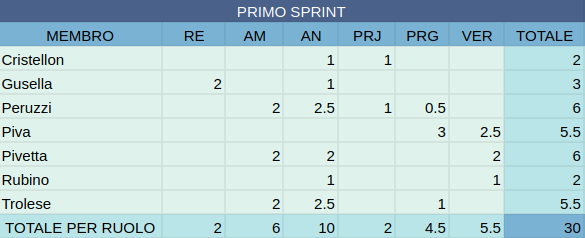
\includegraphics[width=0.6\linewidth]{Consuntivo-table-membri-1.png}
	\caption{Consuntivo orario per membro - primo sprint$_G$}
	\label{fig:Consuntivo orario per membro - primo sprint$_G$}
\end{figure}
\begin{figure}[ht]
	\centering
	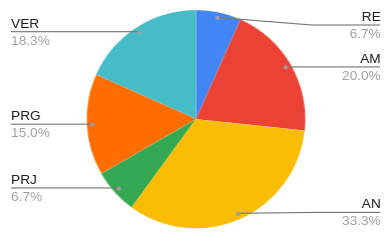
\includegraphics[width=0.4\linewidth]{Consuntivo-ore-ruoli-torta-1.png}
	\caption{Diagramma circolare della partizione delle ore per ruolo - primo sprint$_G$ }
	\label{fig:Diagramma circolare della partizione delle ore per ruolo - primo sprint$_G$}
\end{figure}
\begin{figure}[ht]
	\centering
	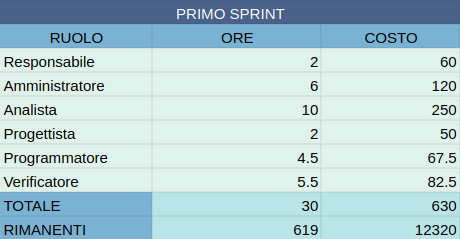
\includegraphics[width=0.6\linewidth]{Consuntivo-table-ruoli-1.png}
	\caption{Consuntivo orario e costi per ruolo - primo sprint$_G$}
	\label{fig:Consuntivo orario e costi per ruolo - primo sprint$_G$}
\end{figure}
\begin{figure}[ht]
	\centering
	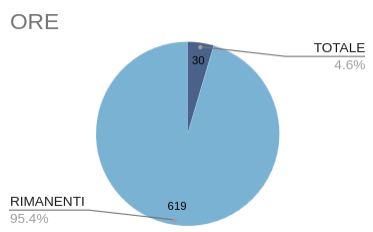
\includegraphics[width=0.5\linewidth]{Consuntivo-ore-tot-torta-1.png}
	\caption{Diagramma circolare delle ore rimanenti - primo sprint$_G$ }
	\label{fig:Diagramma circolare delle ore rimanenti - primo sprint$_G$}
\end{figure}
\begin{figure}[ht]
	\centering
	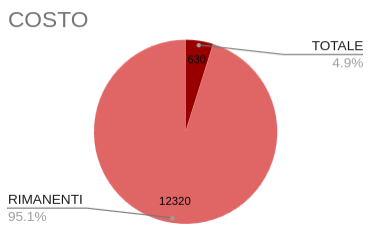
\includegraphics[width=0.5\linewidth]{Consuntivo-costi-tot-torta-1.png}
	\caption{Diagramma circolare dei costi avvenuti - primo sprint$_G$ }
	\label{fig:Diagramma circolare dei costi avvenuti - primo sprint$_G$}
\end{figure}

\end{enumerate}

\end{document}
